\documentclass{beamer}

% To have the citation lists ordered by number.
\usepackage[nocompress]{cite}
\usepackage[utf8]{inputenc}
\usepackage{graphicx}
\usepackage[tight,TABTOPCAP]{subfigure}
\usepackage{amsmath}
\usepackage{amssymb}
\usepackage{amsfonts}
\usepackage{url}
\usepackage{proof}

\usepackage{hyperref}

\usepackage{tikz}
\usetikzlibrary{shapes.symbols}
\usepackage{color}

\usepackage{color}
\usepackage{listings}
\lstset{ %
language=C,                % choose the language of the code
basicstyle=\footnotesize,       % the size of the fonts that are used for the code
numbers=left,                   % where to put the line-numbers
numberstyle=\footnotesize,      % the size of the fonts that are used for the line-numbers
stepnumber=1,                   % the step between two line-numbers. If it is 1 each line will be numbered
numbersep=5pt,                  % how far the line-numbers are from the code
backgroundcolor=\color{white},  % choose the background color. You must add \usepackage{color}
showspaces=false,               % show spaces adding particular underscores
showstringspaces=false,         % underline spaces within strings
showtabs=false,                 % show tabs within strings adding particular underscores
frame=single,   		% adds a frame around the code
tabsize=2,  		% sets default tabsize to 2 spaces
captionpos=b   		% sets the caption-position to bottom
}



%%%%%%%%%% Tool Names %%%%%%%%%%%%
\newcommand{\csisat}{{\sc CSIsat}}
\newcommand{\blast}{{\sc Blast}}
\newcommand{\armc}{{\sc ARMC}}
\newcommand{\mathsat}{{\sc MathSAT}}
\newcommand{\picosat}{{\sc PicoSAT}}
\newcommand{\clpprover}{{\sc CLPprover}}
\newcommand{\foci}{{\sc Foci}}
\newcommand{\sicstus}{{\sc SICStus Prolog}}

%%%%%%%%%% NOTATIONS %%%%%%%%%%%%
\newcommand{\true}{{\it true}}
\newcommand{\false}{{\it false}}
\newcommand{\sat}{{\sc sat}}
\newcommand{\laeuf}{{\sc LA+EUF}}

\renewcommand{\implies}{\Rightarrow}


\mode<presentation>
{
  \usetheme{Warsaw}
  %\usetheme{Frankfurt}
  % or ...

  %\setbeamercovered{transparent}
  % or whatever (possibly just delete it)
  %\setbeamertemplate{footline}[frame number]
  %\useoutertheme{mysplit}
}
% Remove the navigation bar
\setbeamertemplate{navigation symbols}{}

\title[Software Model-Checking]{Software Model-Checking: an algorithmic approach to prove programs correct}

%\AtBeginSection[]
%{
%  \begin{frame}<beamer>
%    \frametitle{Outline}
%    \tableofcontents[currentsection,hideothersubsections]
%  \end{frame}
%}

\author{ Damien Zufferey }

\institute{ IST Austria }
\date{\today}

%-------------------------------------------------------------------------
\begin{document}

% Title
\frame[plain]{\titlepage}

\begin{frame}
  \frametitle{Push-button approach}
\begin{figure}
  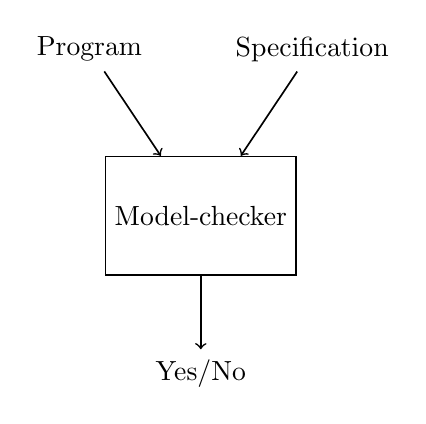
\begin{tikzpicture}[semithick,->,node distance=2cm]
  \node[draw, minimum height=15mm, minimum width=2cm] (MC) at (0,0) {Model-checker};
  \node (prog) [above=7mm, above left of=MC] {Program};
  \node (spec) [above=7mm, above right of=MC] {Specification};
  \node (result) [below of=MC] {Yes/No};
  \path (prog) edge (MC);
  \path (spec) edge (MC);
  \path (MC) edge (result);
  \end{tikzpicture}
\end{figure}
\end{frame}

%\section{Bakery Algorithm}
\begin{frame}
  \frametitle{Running example: Lamport's bakery algorithm}

  There is bakery with only one clerk.
  The clerk can serve only one customer at the time.
  To avoid conflict between customers, a numbering machine gives a ticket to each customer.

  \vspace{10pt}

  What customers do:
  {\small
  \begin{enumerate}
    \item Customer enters the bakery and get a ticket;
    \item If he is alone or has the ticket with lowest number then he orders;
    \item When he is done, he leaves the bakery and throws away the ticket.
  \end{enumerate}
  }

  \vspace{10pt}

  When the bakery is empty the numbering machine is reset.

\end{frame}

\begin{frame}[fragile]
  \frametitle{Implementation of the algorithm for 2 customers.}
\begin{center}
{\footnotesize
initial state: pc1 = 0, x1 = 0, pc2 = 0, x2 = 0\\
pc values: (0 $\rightarrow$ outside), (1 $\rightarrow$ waiting), (2 $\rightarrow$ ordering)
}
\end{center}
\begin{minipage}{0.45\linewidth}
\begin{lstlisting}
while (true) {
  if(pc1 == 0){
    x1 = x2 + 1;
    pc1 = 1;
  }else if(pc1 == 1 &&
            (x2 == 0 ||
             x1 < x2 )){
    pc1 = 2;
  }else if(pc1 == 2){
    pc1 = 0;
    x1 = 0;
  }
  if(pc1==2 && pc2==2){
    ERROR;
  }
}
\end{lstlisting}
\end{minipage}
\hfill
\begin{minipage}{0.45\linewidth}
\begin{lstlisting}
while (true) {
  if(pc2 == 0){
    x2 = x1 + 1;
    pc2 = 1;
  }else if(pc2 == 1 &&
            (x1 == 0 ||
             x2 < x1 )){
    pc2 = 2;
  }else if(pc2 == 2){
    pc2 = 0;
    x2 = 0;
  }
  if(pc1==2 && pc2==2){
    ERROR;
  }
}
\end{lstlisting}
\end{minipage}
\end{frame}

\begin{frame}[fragile]
  \frametitle{Assumptions and model}
  unbounded integers: from $-\infty$ to $\infty$, no overflow.

  \vspace{10pt}

  atomicity: blocks of code are atomic in particular:
\begin{lstlisting}[numbers=none]
  x1 = x2 + 1;
\end{lstlisting}
\begin{lstlisting}[numbers=none]
  if(pc1 == 1 &&
     (x2 == 0 ||
      x1 < x2 )){
    pc1 = 2;
  }
\end{lstlisting}
\end{frame}

\begin{frame}
  \frametitle{Why do we means by correct ?}
  reachability: (safety) no two customers fight.
  
  \vspace{5mm}

  liveness: (starvation-free) every customers eventually get served.

  \vspace{1cm}

  For this talk we will care only about \alert{safety} property.

\end{frame}

\begin{frame}
  \frametitle{General idea:}

\begin{figure}
  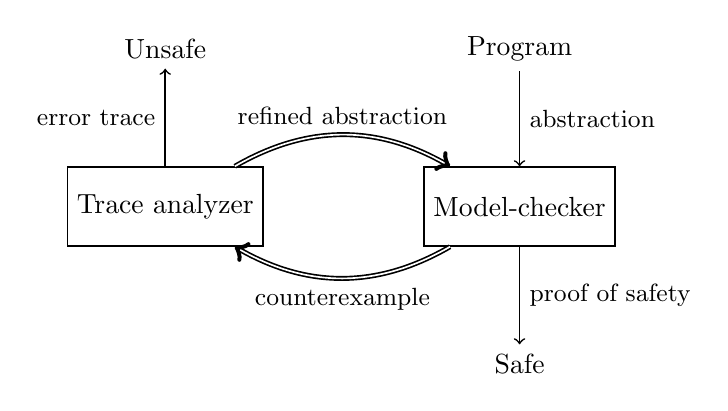
\begin{tikzpicture}[semithick,->,node distance=2cm]
  \node[draw, minimum height=10mm, minimum width=2cm] (MC) at (0,0) {Model-checker};
  \node (prog) [above of=MC] {Program};
  \node (safe) [below of=MC] {Safe};
  \node[draw, minimum height=10mm, minimum width=2cm] (trace) [left=25mm, left of=MC] {Trace analyzer};
  \node (error) [above of=trace] {Unsafe};

  \path (prog) edge node[right] {\small abstraction} (MC);
  \path (MC) edge node[right] {\small proof of safety} (safe);
  \path (MC) edge[double, bend left] node[below] {\small counterexample} (trace);
  \path (trace) edge[double, bend left] node[above] {\small refined abstraction} (MC);
  \path (trace) edge node[left] {\small error trace} (error);
  \end{tikzpicture}
\end{figure}

CEGAR: counterexample guided abstraction refinement

\end{frame}

\begin{frame}[fragile]
  \frametitle{First iteration}

{\footnotesize
predicates: \\
initial state:
}
\vfill
\begin{minipage}{0.45\linewidth}
\begin{lstlisting}
while (true) {
  if(        ){
               ;
           ;
  }else if(         &&
            (        ||
                     )){
           ;
  }else if(        ){
           ;
          ;
  }
  if(       &&       ){
    ERROR;
  }
}
\end{lstlisting}
\end{minipage}
\hfill
\begin{minipage}{0.45\linewidth}
\begin{lstlisting}
while (true) {
  if(        ){
               ;
           ;
  }else if(         &&
            (        ||
                     )){
           ;
  }else if(        ){
           ;
          ;
  }
  if(       &&       ){
    ERROR;
  }
}
\end{lstlisting}
\end{minipage}

\visible<2->{
\begin{tikzpicture}[remember picture, overlay]
  \node (nw) at (current page.north west) {};
  \node (x) [below=12mm, below right of=nw] {};
  \draw[line width=2pt,double,->,color=red!90!black] (x) -- +(0,-4) .. controls +(0,-5) .. +(1,-5.3);
\end{tikzpicture}
}

\visible<3->{
\begin{tikzpicture}[remember picture, overlay]
  \node[text width=6cm, fill=white, draw, very thick] (nw) at (current page.center) {
    pc1 = 0, x1 = 0, pc2 = 0, x2 = 0;\\
    while (true) \{\\
    \mbox{}~~if(pc1==2 \&\& pc2==2)\{\\
    \mbox{}~~~~ERROR;\\
    \mbox{}~~\}\\
    \}
   };
\end{tikzpicture}
}

\end{frame}

\begin{frame}[fragile]
  \frametitle{First counterexample}
\begin{minipage}{0.45\linewidth}
\begin{lstlisting}[numbers=none]
pc1=0, x1=0, pc2=0, x2=0;
assume(pc1==2 && pc2==2);
ERROR;
\end{lstlisting}
\end{minipage}
\vfill
\begin{minipage}{0.8\linewidth}
SSA formula:
\begin{align*}
& \alert<2>{pc_1=0} \land x_1=0 \land pc_2=0 \land x_2=0 \\
& \alert<2>{pc_1=2} \land pc_2=2
\end{align*}
\visible<2>{Formula is unsat $\Rightarrow$ spurious counterexample}
\end{minipage}
\end{frame}

\begin{frame}
  \frametitle{Finding out why the cex is spurious.}

  Let $A$ and $B$ be two formulas such that
  $A \wedge B$ unsat.\\
  A [Craig] interpolant $I$ has the following properties:
  \begin{itemize}
  \item $I$ contains only $AB$-common symbols.
  \item $A$ implies $I$
  \item $I \wedge B$ unsat.
  \end{itemize}

\begin{align*}
& pc_1=0 \land x_1=0 \land pc_2=0 \land x_2=0 \\
& \hspace{8cm} \visible<2->{\alert{pc_1 = 0}}\\
& pc_1=2 \land pc_2=2
\end{align*}
\end{frame}

\begin{frame}[fragile]
  \frametitle{Second iteration}

{\footnotesize
predicates: pc1 = 0\\
initial state: pc1 = 0
}
\vfill
\begin{minipage}{0.45\linewidth}
\begin{lstlisting}
while (true) {
  if(pc1 == 0){
               ;
    pc1 = 1;
  }else if(pc1 == 1 &&
            (        ||
                     )){
    pc1 = 2;
  }else if(pc1 == 2){
    pc1 = 0;
          ;
  }
  if(pc1==2 &&       ){
    ERROR;
  }
}
\end{lstlisting}
\end{minipage}
\hfill
\begin{minipage}{0.45\linewidth}
\begin{lstlisting}
while (true) {
  if(        ){
               ;
           ;
  }else if(         &&
            (        ||
                     )){
           ;
  }else if(        ){
           ;
          ;
  }
  if(pc1==2 &&       ){
    ERROR;
  }
}
\end{lstlisting}
\end{minipage}

\visible<2>{
\begin{tikzpicture}[remember picture, overlay]
  \node (nw) at (current page.north west) {};
  \node (x) [below=15mm, below right of=nw] {};
  \draw[line width=2pt,double,->,color=red!90!black] (x) .. controls +(2,-0.75) .. +(0,-1.5) -- +(0,-4) .. controls +(0,-5) .. +(1,-5.3);
\end{tikzpicture}
}
\end{frame}

\begin{frame}[fragile]
  \frametitle{Second counterexample}
\begin{minipage}{0.45\linewidth}
\begin{lstlisting}[numbers=none]
pc1=0, x1=0, pc2=0, x2=0;
assume(pc1 == 0);
x1 = x2 + 1;
pc1 = 1;
assume(pc1==2 && pc2==2);
ERROR;
\end{lstlisting}
\end{minipage}
\vfill
\begin{minipage}{0.8\linewidth}
SSA formula:
\begin{align*}
& pc_1=0 \land x_1=0 \land pc_2=0 \land x_2=0 \\
& pc_1=0 \\
& x_1' = x_2 + 1 \\
& \alert<2>{pc_1' = 1} \\
& \alert<2>{pc_1'=2} \land pc_2=2
\end{align*}
\visible<2>{Formula is unsat $\Rightarrow$ spurious counterexample}
\end{minipage}
\end{frame}

\begin{frame}
  \frametitle{Finding out why the cex is spurious.}

\begin{align*}
& pc_1=0 \land x_1=0 \land pc_2=0 \land x_2=0 \\
& \hspace{8cm} \visible<2->{\top} \\
& pc_1=0 \\
& \hspace{8cm} \visible<3->{\top} \\
& x_1' = x_2 + 1 \\
& \hspace{8cm} \visible<4->{\top} \\
& pc_1' = 1 \\
& \hspace{8cm} \visible<5->{pc_1' = 1}\\
& pc_1'=2 \land pc_2=2
\end{align*}
\end{frame}

\begin{frame}[fragile]
  \frametitle{Third iteration}

{\footnotesize
predicates: pc1 = 0, pc1 = 1\\
initial state: pc1 = 0
}
\vfill
\begin{minipage}{0.45\linewidth}
\begin{lstlisting}
while (true) {
  if(pc1 == 0){
               ;
    pc1 = 1;
  }else if(pc1 == 1 &&
            (        ||
                     )){
    pc1 = 2;
  }else if(pc1 == 2){
    pc1 = 0;
          ;
  }
  if(pc1==2 &&       ){
    ERROR;
  }
}
\end{lstlisting}
\end{minipage}
\hfill
\begin{minipage}{0.45\linewidth}
\begin{lstlisting}
while (true) {
  if(        ){
               ;
           ;
  }else if(         &&
            (        ||
                     )){
           ;
  }else if(        ){
           ;
          ;
  }
  if(pc1==2 &&       ){
    ERROR;
  }
}
\end{lstlisting}
\end{minipage}

\begin{tikzpicture}[remember picture, overlay]
  \node (nw) at (current page.north west) {};
  \node (x) [below=15mm, below right of=nw] {};
  \node (y) [right of=x] {};
  \visible<2->{ \draw[line width=2pt,double,->,color=red!90!black] (x) .. controls +(1,-0.75) .. +(0,-1.5) -- +(0,-6); }
  \visible<3->{ \draw[line width=2pt,double,->,color=red!90!black] (y) -- +(0,-2) .. controls +(1,-2.5) .. +(0,-3) .. controls +(0,-5) .. +(1,-5.3); }
\end{tikzpicture}
\end{frame}

\begin{frame}[fragile]
  \frametitle{Third counterexample}
\begin{minipage}{0.65\linewidth}
\begin{lstlisting}[numbers=none]
pc1=0, x1=0, pc2=0, x2=0;
assume(pc1 == 0);
x1 = x2 + 1;
pc1 = 1;
assume(pc1==1 && (x1==0 || x2<x1));
pc1 = 2;
assume(pc1==2 && pc2==2);
ERROR;
\end{lstlisting}
\end{minipage}
\begin{minipage}{0.8\linewidth}
\begin{align*}
& pc_1=0 \land x_1=0 \land \alert<2>{pc_2=0} \land x_2=0 \\
& pc_1=0 \\
& x_1' = x_2 + 1 \\
& pc_1' = 1 \\
& pc_1'=1 \land (x_2=0 \lor x_1'<x_2) \\
& pc_1'' = 2 \\
& pc_1''=2 \land \alert<2>{pc_2=2}
\end{align*}
\visible<2>{Formula is unsat $\Rightarrow$ spurious counterexample}
\end{minipage}
\end{frame}

\begin{frame}[fragile]
  \frametitle{A few iterations later ...}

{\footnotesize
predicates: pc1 = 0, pc1 = 1, pc2 = 0, pc2 = 1\\
initial state: pc1 = 0, pc2 = 0
}
\vfill
\begin{minipage}{0.45\linewidth}
\begin{lstlisting}
while (true) {
  if(pc1 == 0){
               ;
    pc1 = 1;
  }else if(pc1 == 1 &&
            (        ||
                     )){
    pc1 = 2;
  }else if(pc1 == 2){
    pc1 = 0;
          ;
  }
  if(pc1==2 && pc2==2){
    ERROR;
  }
}
\end{lstlisting}
\end{minipage}
\hfill
\begin{minipage}{0.45\linewidth}
\begin{lstlisting}
while (true) {
  if(pc2 == 0){
               ;
    pc2 = 1;
  }else if(pc2 == 1 &&
            (        ||
                     )){
    pc2 = 2;
  }else if(pc2 == 2){
    pc2 = 0;
          ;
  }
  if(pc1==2 && pc2==2){
    ERROR;
  }
}
\end{lstlisting}
\end{minipage}

\begin{tikzpicture}[remember picture, overlay]
  \node (nw) at (current page.north west) {};
  \node (x) [below=15mm, below right of=nw] {};
  \node (y) [right of=x] {};
  \node (n) at (current page.north) {};
  \node (z) [below=12mm, below of=n] {};
  \node (a) [right of=z] {};
\visible<2->{ \draw[line width=2pt,double,->,color=red!90!black] (x) .. controls +(1,-0.75) .. +(0,-1.5) -- +(0,-6);}
\visible<3->{ \draw[line width=2pt,double,->,color=red!90!black] (y) -- +(0,-2) .. controls +(1,-2.5) .. +(0,-3) -- +(0,-6);}
\visible<4->{ \draw[line width=2pt,double,->,color=red!90!black] (z) .. controls +(1,-0.75) .. +(0,-1.5) -- +(0,-6);}
\visible<5->{ \draw[line width=2pt,double,->,color=red!90!black] (a) -- +(0,-2) .. controls +(1,-2.5) .. +(0,-3) .. controls +(0,-5) .. +(1,-5.3);}
\end{tikzpicture}
\end{frame}

\begin{frame}
  \frametitle{Finding out why the cex is spurious (first possibility)}

\begin{align*}
& pc_1=0 \land x_1=0 \land pc_2=0 \land x_2=0 \\
& \hspace{8cm} \visible<2->{x_2=0} \\
& pc_1=0 \land x_1' = x_2 + 1 \land pc_1' = 1 \\
& \hspace{8cm} \visible<3->{x_1' = 1 \land x_2 = 0} \\
& pc_1'=1 \land (x_2=0 \lor x_1'<x_2) \land pc_1'' = 2 \\
& \hspace{8cm} \visible<4->{x_1' = 1}\\
& pc_2=0 \land x_2' = x_1' + 1 \land pc_2' = 1 \\
& \hspace{8cm} \visible<5->{x_1' = 1 \land x_2' = 2} \\
& pc_2'=1 \land (x_1'=0 \lor x_2'<x_1') \land pc_2'' = 2 \\
& \hspace{8cm} \visible<6->{\bot}\\
& pc_1''=2 \land pc_2''=2
\end{align*}
\end{frame}


\begin{frame}[fragile]
  \frametitle{Does it work ?}

{\footnotesize
predicates: pc1 = 0, pc1 = 1, pc2 = 0, pc2 = 1, x1=1, x2=0, x2=2\\
initial state: pc1 = 0, x1 = 0, pc2 = 0, x2 = 0
}
\vfill
\begin{minipage}{0.45\linewidth}
\begin{lstlisting}
while (true) {
  if(pc1 == 0){
    x1 = x2 + 1;
    pc1 = 1;
  }else if(pc1 == 1 &&
            (x2 == 0 ||
             x1 < x2 )){
    pc1 = 2;
  }else if(pc1 == 2){
    pc1 = 0;
    x1 = 0;
  }
  if(pc1==2 && pc2==2){
    ERROR;
  }
}
\end{lstlisting}
\end{minipage}
\hfill
\begin{minipage}{0.45\linewidth}
\begin{lstlisting}
while (true) {
  if(pc2 == 0){
    x2 = x1 + 1;
    pc2 = 1;
  }else if(pc2 == 1 &&
            (x1 == 0 ||
             x2 < x1 )){
    pc2 = 2;
  }else if(pc2 == 2){
    pc2 = 0;
    x2 = 0;
  }
  if(pc1==2 && pc2==2){
    ERROR;
  }
}
\end{lstlisting}
\end{minipage}

\begin{tikzpicture}[remember picture, overlay]
  \node (nw) at (current page.north west) {};
  \node (x1) [below=15mm, below right of=nw] {};
  \node (x2) [right of=x1] {};
  \node (x3) [right of=x2] {};
  \node (x4) [right of=x3] {};
  \node (x5) [right of=x4] {};
  \node (n) at (current page.north) {};
  \node (y1) [below=12mm, below of=n] {};
  \node (y2) [right of=y1] {};
  \node (y3) [right of=y2] {};
  \node (y4) [right of=y3] {};
  \node (y5) [right of=y4] {};
\visible<2->{ \draw[line width=2pt,double,->,color=red!90!black] (x1) .. controls +(1,-0.75) .. +(0,-1.5) -- +(0,-6); }
\visible<3->{ \draw[line width=2pt,double,->,color=red!90!black] (x2) -- +(0,-2) .. controls +(1,-2.5) .. +(0,-3) -- +(0,-6);}
\visible<4->{ \draw[line width=2pt,double,->,color=red!90!black] (y1) .. controls +(1,-0.75) .. +(0,-1.5) -- +(0,-6);}
\visible<5->{ \draw[line width=2pt,double,->,color=red!90!black] (x3) -- +(0,-3.5) .. controls +(1,-4) .. +(0,-4.5) -- +(0,-6);}
\visible<6->{ \draw[line width=2pt,double,->,color=red!90!black] (x4) .. controls +(1,-0.75) .. +(0,-1.5) -- +(0,-6); }
\visible<7->{ \draw[line width=2pt,double,->,color=red!90!black] (y2) -- +(0,-2) .. controls +(1,-2.5) .. +(0,-3) -- +(0,-6);}
\visible<8->{ \draw[line width=2pt,double,->,color=red!90!black] (y3) -- +(0,-3.5) .. controls +(1,-4) .. +(0,-4.5) -- +(0,-6);}
\visible<9->{ \draw[line width=2pt,double,->,color=red!90!black] (y4) .. controls +(1,-0.75) .. +(0,-1.5) -- +(0,-6); }
\visible<10->{ \draw[line width=2pt,double,->,color=red!90!black] (x5) -- +(0,-2) .. controls +(1,-2.5) .. +(0,-3) -- +(0,-6);}
\visible<11->{ \draw[line width=2pt,double,->,color=red!90!black] (y5) -- +(0,-2) .. controls +(1,-2.5) .. +(0,-3) .. controls +(0,-5) .. +(1,-5.3);}
\end{tikzpicture}
\end{frame}

\begin{frame}
  \frametitle{Finding out why the cex is spurious (second possibility)}

\begin{align*}
& pc_1=0 \land x_1=0 \land pc_2=0 \land x_2=0 \\
& \hspace{8cm} \visible<2->{x_2=0} \\
& pc_1=0 \land x_1' = x_2 + 1 \land pc_1' = 1 \\
& \hspace{8cm} \visible<3->{x_1' > x_2 \land x_2 = 0} \\
& pc_1'=1 \land (x_2=0 \lor x_1'<x_2) \land pc_1'' = 2 \\
& \hspace{8cm} \visible<4->{x_1' > 0}\\
& pc_2=0 \land x_2' = x_1' + 1 \land pc_2' = 1 \\
& \hspace{8cm} \visible<5->{x_1' > 0 \land x_2' > x_1'} \\
& pc_2'=1 \land (x_1'=0 \lor x_2'<x_1') \land pc_2'' = 2 \\
& \hspace{8cm} \visible<6->{\bot}\\
& pc_1''=2 \land pc_2''=2
\end{align*}
\end{frame}

\begin{frame}[fragile]
  \frametitle{Final version}

{\footnotesize
predicates: pc1=0, pc1=1, pc2=0, pc2=1, x1=0, x2=0, x1$<$x2, x1$>$x2\\
initial state: pc1 = 0, x1 = 0, pc2 = 0, x2 = 0
}
\vfill
\begin{minipage}{0.45\linewidth}
\begin{lstlisting}
while (true) {
  if(pc1 == 0){
    x1 = x2 + 1;
    pc1 = 1;
  }else if(pc1 == 1 &&
            (x2 == 0 ||
             x1 < x2 )){
    pc1 = 2;
  }else if(pc1 == 2){
    pc1 = 0;
    x1 = 0;
  }
  if(pc1==2 && pc2==2){
    ERROR;
  }
}
\end{lstlisting}
\end{minipage}
\hfill
\begin{minipage}{0.45\linewidth}
\begin{lstlisting}
while (true) {
  if(pc2 == 0){
    x2 = x1 + 1;
    pc2 = 1;
  }else if(pc2 == 1 &&
            (x1 == 0 ||
             x2 < x1 )){
    pc2 = 2;
  }else if(pc2 == 2){
    pc2 = 0;
    x2 = 0;
  }
  if(pc1==2 && pc2==2){
    ERROR;
  }
}
\end{lstlisting}
\end{minipage}
\end{frame}

\begin{frame}
  \frametitle{Building an actual proof}
  state-space: 2 * 16 loc and 8 predicates $\Rightarrow 16^2 * 2^8 = 65536$ states

  \vfill

  \visible<2>{
  simpler version:

  {\scriptsize
  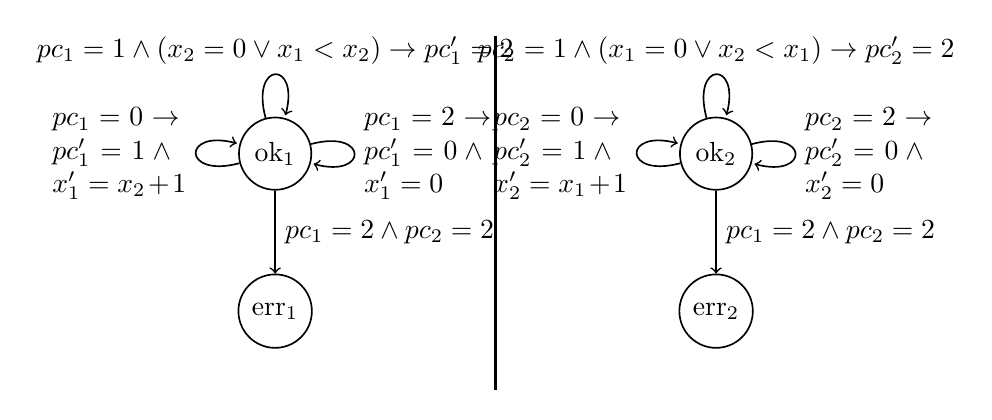
\begin{tikzpicture}[semithick, node distance=2cm]
  \begin{scope}[xshift=-28mm]
  \node[draw,circle]  (o) at (0,0) {ok$_1$};
  \node[draw,circle]  (e) [below of=o] {err$_1$};
  \path  (o) edge [loop left] node[left,text width=1.7cm] {$pc_1=0 \rightarrow pc_1'=1 \land x_1' = x_2 + 1$} (o)
         (o) edge [loop above] node[above] {$pc_1=1 \land (x_2=0 \lor x_1<x_2) \rightarrow pc_1'=2$} (o)
         (o) edge [loop right] node[right,text width=1.7cm] {$pc_1=2 \rightarrow pc_1' = 0 \land x_1' = 0$}(o)
         (o) edge[->] node[right] {$pc_1=2 \land pc_2=2$} (e);
  \end{scope}
  \draw[very thick] (0,1.5) -- (0,-3);
  \begin{scope}[xshift=28mm]
  \node[draw,circle]  (o) at (0,0) {ok$_2$};
  \node[draw,circle]  (e) [below of=o] {err$_2$};
  \path  (o) edge [loop left] node[left,text width=1.7cm] {$pc_2=0 \rightarrow pc_2'=1 \land x_2' = x_1 + 1$} (o)
         (o) edge [loop above] node[above] {$pc_2=1 \land (x_1=0 \lor x_2<x_1) \rightarrow pc_2'=2$} (o)
         (o) edge [loop right] node[right,text width=1.7cm] {$pc_2=2 \rightarrow pc_2' = 0 \land x_2' = 0$}(o)
         (o) edge[->] node[right] {$pc_1=2 \land pc_2=2$} (e);
  \end{scope}
  \end{tikzpicture}
  }
  state-space: $2^2 * 2^8 = 1024$ states

  By being clever with the predicates we can go down to 432 states (12 are reachable).
  }

\end{frame}

\begin{frame}
  \frametitle{Reachability graph}

\begin{minipage}{0.65\linewidth}
{\small
\begin{tabular}{l|ccccc}
id & pc1 & pc2 & $x_1=0$ & $x_2=0$ & $x_1 ? x_2$ \\
\hline
0  & 0  &  0  &  $\top$ & $\top$ & $x_1 = x_2$ \\
1  & 1  &  0  &  $\bot$ & $\top$ & $x_1 > x_2$ \\
2  & 0  &  1  &  $\top$ & $\bot$ & $x_1 < x_2$ \\
3  & 1  &  1  &  $\bot$ & $\bot$ & $x_1 < x_2$ \\
4  & 2  &  0  &  $\bot$ & $\top$ & $x_1 > x_2$ \\
5  & 0  &  2  &  $\top$ & $\bot$ & $x_1 < x_2$ \\
6  & 1  &  1  &  $\bot$ & $\bot$ & $x_1 > x_2$ \\
7  & 2  &  1  &  $\bot$ & $\bot$ & $x_1 < x_2$ \\
8  & 1  &  2  &  $\bot$ & $\bot$ & $x_1 > x_2$ \\
9  & 0  &  1  &  $\top$ & $\bot$ & $x_1 > x_2$ \\
10 & 1  &  0  &  $\bot$ & $\top$ & $x_1 < x_2$ \\
11 & 0  &  2  &  $\top$ & $\bot$ & $x_1 > x_2$ \\
12 & 2  &  0  &  $\bot$ & $\top$ & $x_1 < x_2$
\end{tabular}
}
\end{minipage}
\begin{minipage}{0.3\linewidth}
  \includegraphics[scale=0.3]{rg}
\end{minipage}

\end{frame}

\begin{frame}
  \frametitle{Why is it a proof ?}

  \begin{figure}
  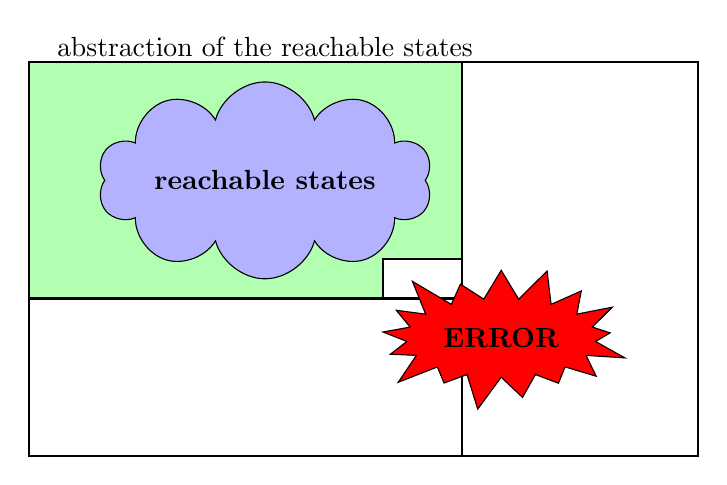
\begin{tikzpicture}
    \visible<2->{\node at (0,1.7) {abstraction of the reachable states};}
    \visible<2>{\draw[thick] (-3,1.5) rectangle (5.5,-3.5);}
    \visible<3>{\draw[thick] (-3,1.5) rectangle (2.5,-3.5);}
    \visible<4>{\draw[thick] (-3,1.5) rectangle (2.5,-1.5);}
    \visible<5>{\path[draw, thick] (-3,1.5) -- (-3, -1.5) -- (1.5,-1.5) -- (1.5,-1) -- (2.5,-1) -- (2.5,1.5) -- cycle;}
    \visible<6>{\path[draw, thick, fill=green!30] (-3,1.5) -- (-3, -1.5) -- (1.5,-1.5) -- (1.5,-1) -- (2.5,-1) -- (2.5,1.5) -- cycle;}
    \node[cloud, cloud ignores aspect, draw, minimum width=3cm, minimum height=25mm, fill=blue!30] at (0,0) {\bf reachable states};
    \node[starburst, draw, fill=red, minimum width=3cm, minimum height=2cm] at (3,-2) {\bf ERROR};
  \end{tikzpicture}
  \end{figure}


  %Galois connection

  %inductive invariant

\end{frame}


%\section*{Conclusion}
\begin{frame}

\begin{center}
\Huge
Questions ?
\end{center}
\end{frame}


\end{document}
